\clearpage
\scanpage{5}
\figure{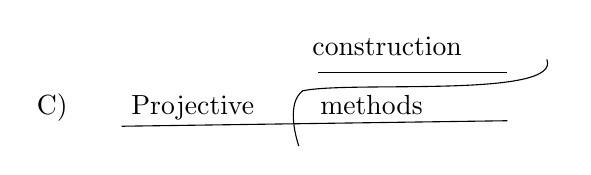
\begin{tikzpicture}[every node/.style={anchor=base west}]
\node at (0,0) {C)};
\node at (1.2,0) {Projective};\node at (3.6,0) {methods};
\node at (3.5,.75) {\inserted{construction}};
\draw (1.2,-.15)--(6.1,-.08);\draw (3.7,.53)--(6.1,.53);
\draw (6.6,.7)..controls (6.8,.2) and (4.1,.43)..(3.5,.3)..controls (3.3,.15) and (3.4,-.25)..(3.45,-.4);
\end{tikzpicture}}

\S\,14\quad Bounded families.

\figure{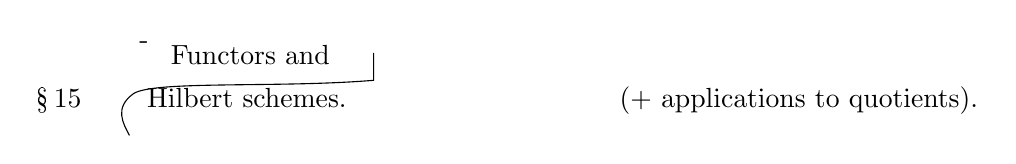
\begin{tikzpicture}[every node/.style={anchor=base west}]
\node at (0,0) {\S\,15};\node at (1.4,0) {Hilbert schemes.};\node at (7.4,0) {(+ applications to quotients).};
\node at (1.7,.55) {\inserted{Functors and}};\node at (1.3,.75) {\unsure{-}};
\draw (4.4,.7)--(4.4,.35)..controls (3.2,.25) and (1.6,.35)..(1.35,.18)..controls (1.1,0) and (1.22,-.2)..(1.3,-.35);
\end{tikzpicture}}

\figure{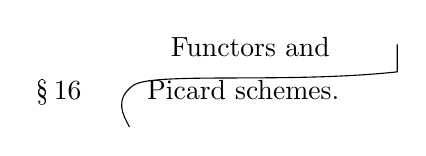
\begin{tikzpicture}[every node/.style={anchor=base west}]
\node at (0,0) {\S\,16};\node at (1.4,0) {Picard schemes.};
\node at (1.7,.55) {\inserted{Functors and}};
\draw (4.7,.7)--(4.7,.35)..controls (3.3,.2) and (1.6,.35)..(1.35,.18)..controls (1.1,0) and (1.22,-.2)..(1.3,-.35);
\end{tikzpicture}}
\margin{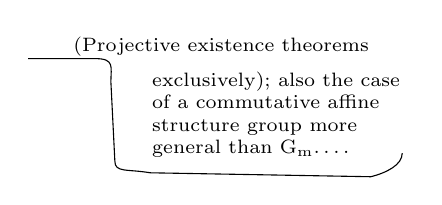
\begin{tikzpicture}[every node/.style={anchor=north west,font=\scriptsize,align=left}]
\node[text width=4cm] at (0,0) {(Projective existence theorems};
\node[text width=3.2cm] at (1,-.45) {exclusively\deleted{\unsure{)}}; also the case of a commutative affine structure group more general than $\mathrm G_{\mathrm m}$\ldots.};
\draw (-.45,-.4)--(.4,-.4)..controls (.65,-.4) and (.6,-.5)..(.6,-.7)--(.65,-1.7)..controls (.65,-1.85) and (.8,-1.8)..(1.1,-1.85)--(3.9,-1.9)..controls (4.1,-1.85) and (4.3,-1.75)..(4.3,-1.6);
\end{tikzpicture}}

\S\,17\quad Variants of Picard.

\S\,1\deleted{\unsure{7}}8\quad Applications to curves

\S\,1\deleted{\unsure{8}}\unsure{9|8}\quad Formalism of norms

\S\,\deleted{\unsure{19}}20\quad Mumford's multiprojective invariants.

\figure{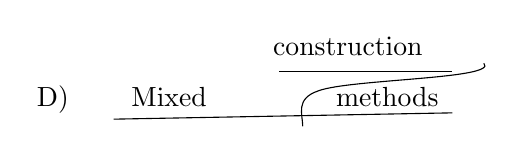
\begin{tikzpicture}[every node/.style={anchor=base west}]
\node at (0,0) {D)};\node at (1.2,0) {Mixed};\node at (3.8,0) {methods};
\node at (3,.65) {\inserted{construction}};
\draw (1.1,-.16)--(5.4,-.08);\draw (3.2,.45)--(5.4,.45);
\draw (5.8,.55)..controls (6,.35) and (4.1,.35)..(3.7,.2)..controls (3.4,.1) and (3.5,-.1)..(3.5,-.25);
\end{tikzpicture}}

\S\,2\deleted{0}1\quad Cases of representability of $\mathrm P\underline{\mathrm{ic}}$, $\mathrm P\underline{\mathrm i\unsure{\mathrm c|\mathrm e}}^{\unsure{0|o|\circ}}$, $\unsure{-|\deleted{\mathrm P}}\mathrm P\underline{\mathrm{ic}}_{X}^{\tau}$ \ldots

(including Mumford's case using \S\,\deleted{\unsure{19}}20).

\S\,21\quad Cases of representability of the functors $\prod_{\deleted{X}Y/S}X/Y$ and so on.

(\unsure{theorems|Theorems} of Matsumura type).

\noindent\rule{\linewidth}{.3pt}

NB.\quad We assume \unsure{known|known} all the functorial \unsure{generalities} (topologies, descent sheaves, \unsure{quotients|quotient}) ; to be recalled if necessary in $\unsure{0|O}_{\underline{\overline{\mathrm V}}}$.

\noindent\rule{\linewidth}{.3pt}

\uline{Missing} :

\figure{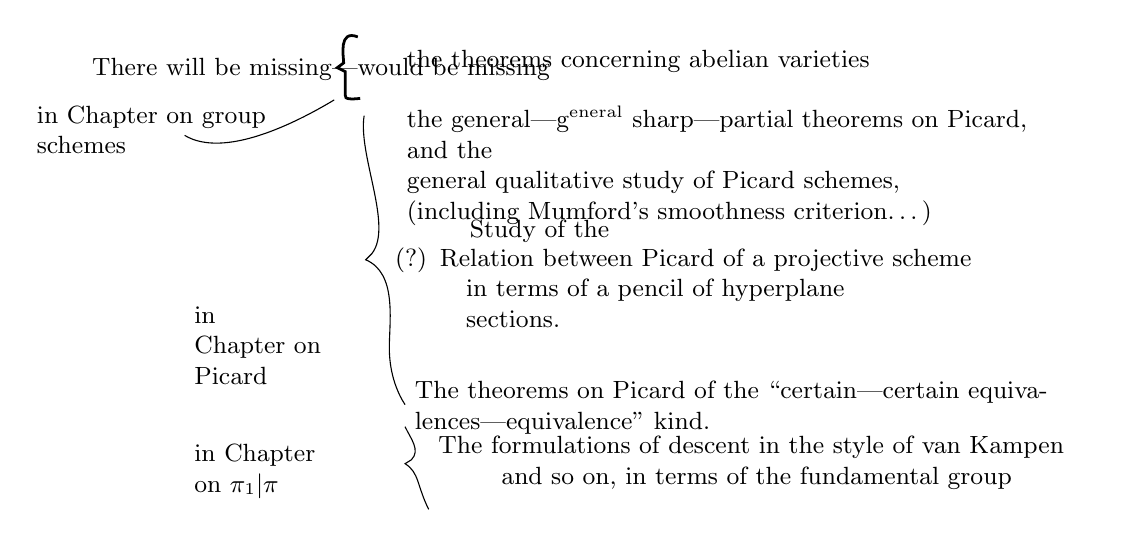
\begin{tikzpicture}[every node/.style={anchor=north west,align=left,font=\small}]
\node at (.7,0) {\deleted{There \unsure{will be missing|would be missing}}};
\node[text width=3.6cm] at (0,-.6) {in Chapter on group\\schemes};
\node at (4.7,.1) {the theorems concerning abelian varieties};
\node[text width=8.3cm] at (4.7,-.6) {the \unsure{general|g\textsuperscript{eneral}} \unsure{sharp|partial} theorems on Picard, and the\\general qualitative study of Picard schemes,\\(including Mumford's smoothness criterion\ldots)};
\draw[line width=1pt] (4.2,.15)..controls (3.95,.25) and (4.02,-.1)..(4.02,-.18)--(3.94,-.24)--(4.04,-.29)--(4.04,-.59)..controls (4.02,-.65) and (4.15,-.64)..(4.23,-.63);
\draw (2,-1.1)..controls (2.5,-1.4) and (3.4,-.95)..(3.9,-.65);
\node[text width=2.2cm] at (2,-3.15) {in\\Chapter on\\Picard};
\draw (4.28,-.85)..controls (4.2,-1.35) and (4.65,-2.25)..(4.38,-2.6)--(4.3,-2.68)..controls (4.7,-2.85) and (4.6,-3.45)..(4.6,-3.8)..controls (4.6,-4.15) and (4.72,-4.4)..(4.8,-4.52);
\node at (5.5,-2.05) {\inserted{Study of the}};
\node[text width=8.8cm] at (4.55,-2.4) {(?) \deleted{\unsure{Relation} between} Picard of a projective scheme\\\hspace*{.9cm}in terms of a pencil of hyperplane\\\hspace*{.9cm}sections.};
\node[text width=8.4cm] at (4.8,-4.1) {The theorems on Picard of the ``\unsure{certain|certain} \unsure{equivalences|equivalence}'' kind.};
\node[text width=2.4cm] at (2,-4.9) {in Chapter\\on $\unsure{\pi_1|\pi}$};
\draw (4.8,-4.8)..controls (4.87,-4.95) and (5,-5.1)..(4.88,-5.22)--(4.8,-5.27)..controls (4.98,-5.38) and (4.95,-5.55)..(5.1,-5.85);
\node[text width=8.2cm] at (5.1,-4.8) {The formulations of descent in the style of van Kampen\\\hspace*{.8cm}and so on, in terms of the fundamental group};
\end{tikzpicture}}
% archive sheet number: 4
